\chapter{Výběr algoritmu pro detekci klíčových bodů}
\label{chap:Pose}

Jelikož je dnes dostupných mnoho různých algoritmů či natrénovaných modelů pro
detekci pózy osob v obrázku či videu, nemá smysl pro navrhované řešení
implementovat takovýto algoritmus od nuly. Možné by to samozřejmě bylo, i
vzhledem k dostupnosti otevřených trénovacích dat (např. dataset COCO
\cite{coco}), nicméně by pravděpodobně nebylo dosaženo tak kvalitních výsledků,
jako řešení, která jsou výsledkem mnoholetých výzkumů. Hlavně pak by bylo těžko
dosáhnout výkonu těchto řešení, a ten je pro navrhované řešení stěžejní,
jelikož je potřeba video zpracovávat v reálném čase.

V následující kapitole budou popsány obecné principy detekce osob a jejich pózy
v obraze. Následně budou popsány některé populární algoritmy pro detekci pózy
se zaměřením na jejich specifika. Několik z nich pak bude otestováno, výsledky
budou porovnány, a na jejich základě bude zvolen algoritmus použitý v konečném
řešení detekce pádu.

\section{Detekce pózy}

\begin{figure}[]
    \centering
    \begin{minipage}{0.48\textwidth}
        \centering
        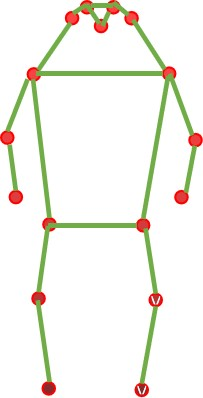
\includegraphics[width=0.5\textwidth]{Figures/keypoints.png}
    \end{minipage}
    \hfill
    \begin{minipage}{0.48\textwidth}
        \centering
        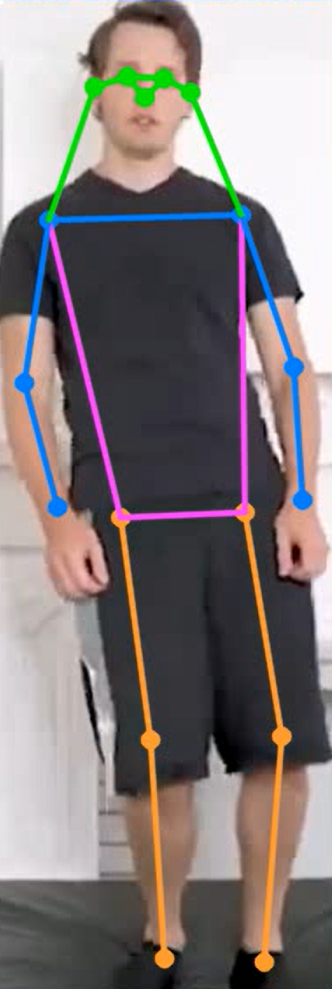
\includegraphics[width=0.35\textwidth]{Figures/pose1.png}
    \end{minipage}
    \caption{(Vlevo) Topologie klíčových bodů použitá např. v COCO-pose \cite{2dhpe} (Vpravo) Příklad detekce pózy pomocí YOLO.}
    \label{fig:keypoints}
\end{figure}

Úloha detekce pózy spočívá v nalezení klíčových bodů postavy v obraze.
% Může se
% jednat také o zvíře, v našem případě se ale budeme zabývat pouze klíčovými body
% lidské postavy. 
Klíčové body představují důležité body lidského těla, znalost jejich lokalizace
nám umožňuje analyzovat pózu dané osoby, popřípadě sledovat její pohyb. K
základním klíčovým bodům patří hlava, ramena, lokty, zápěstí, kyčle, kolena a
kotníky, viz obrázek \ref{fig:keypoints}. Některé algoritmy dokážou rozeznat i
orientaci dlaně či stopy, nebo rozpoznat klíčové body na hlavě, jako jsou ústa,
nos, oči a uši \cite{blazepose}.

Klíčové body jsou většinou reprezentovány jako dvojice souřadnic $(x, y)$
vzhledem k celému obrazu, některé algoritmy poskytují i souřadnice
normalizované vzhledem k bounding boxu osoby. Existují také algoritmy pro 3D
souřadnice, těmto ale nebude věnována pozornost, i když by mohly stanovit
zajímavou alternativu, zejména pokud by pro detekci bylo použito více kamer z
různých pohledů.

V oblasti algoritmů pro detekci pózy existují dva základní přístupy: zdola
nahoru a shora dolů. Přístup zdola nahoru se snaží detekovat všechny klíčové
body v obraze, aniž by rozlišoval jednotlivé osoby, pokud je algoritmus schopen
detekce pózy pro více osob, pak v dalším kroku tyto body spojuje do
jednotlivých postav. Naproti tomu přístup shora dolů nejprve detekuje všechny
osoby v obraze, v jejich rámci pak detekuje klíčové body.

%todo 
\section{Detekce klíčových bodů}

\subsubsection*{Heatmapy}

U obou výše zmíněných přístupů se nejčastěji provádí vyhledání všech klíčových
bodů pomocí tzv. heatmap. Je to 2D mapa pravděpodobnosti, že se v daném bodě
vyskytuje nějaký klíčový bod. Maximální hodnoty v této mapě pak představují
lokalizaci klíčových bodů.

Pro vygenerování heatmap se používá konvoluční neuronová síť. Pro každý klíčový
bod, resp. pro každý typ klíčového bodu k (v případě detekce pózy více osob)
vzniká jedna heatmapa. Jako referenční heatmapy pro trénování se používají
mapy, kde je klíčový bod reprezentován 2D Gaussovým rozložením s vrcholem v
místě daného bodu.

V dalším kroku jsou z heatmap vygenerovány, nejčastěji s pomocí algoritmu
argmax, souřadnice klíčových bodů. V případě vícero osob je pak třeba tyto body
spojit do jednotlivých osob.

\subsubsection*{Regrese}

Využití heatmap je velmi přesné, nicméně z důvodu nutnosti provádění dvou
sekvenčních výpočtů je trochu pomalé. Heatmapy také komplikují proces
trénování, jelikož je třeba spolu s trénovacími daty dodat modelu i heatmapy.
Některé algoritmy se proto snaží formulovat úlohu jako regresi vedoucí přímo k
souřadnicím klíčových bodů. Tento přístup je ve své podstatě trochu méně
přesný, nicméně je rychlejší.

Vůbec první algoritmus pro detekci pózy využívající hluboké učení, DeepPose
\cite{deeppose}, který byl vytvořen v roce 2014 společností Google, používal
právě regresi. Také algoritmus YOLO používá regresi pro určení souřadnic
klíčových bodů, nicméně detekce je prováděná pro detekované objekty, nikoliv
nad celým vstupním obrazem \cite{yolo-pose}.

% , a je součástí poupraveného modelu pro detekci objektů – v posledních
% vrstvách sítě je kromě regrese definující bounding box a klasifikace určující
% třídu prováděna regrese pro určení klíčových bodů.

\section{Detekce objektů a osob v obraze}
\label{sec:obj_det}

Detekce osob se v podstatě může generalizovat na detekci objektů v obraze.
Detekci objektů v obraze definujeme jako úlohu, kdy ve vstupním obrázku určíme
lokalizaci a třídu všech hledaných objektů. Lokalizace je většinou
reprezentována jako souřadnice obdélníku ohraničujícího daný objekt, tzv.
bounding box.

V kapitole \ref{chap:CNN} byla popsána základní architektura konvolučních
neuronových sítí, ta se ale většinou v praxi používá pro klasifikaci obrázků,
nikoliv pro detekci objektů – algoritmus tedy pouze určí, o jakou třídu objektu
se jedná, a ideálně potřebuje, aby objekt vyplňoval celý vstupní obraz.
Teoreticky by bylo možné detekci formulovat jako regresní problém a natrénovat
takovou síť, která by pomocí několika konvolučních vrstev následovaných
několika plně propojenými vrstvami byla schopna predikovat lokalizaci a třídu
všech objektů v obraze \cite{szegedy}. Problém detekce je ale velice komplexní
a také by vyžadoval velice komplexní síť – více vrstev s mnoha filtry, resp.
neurony. Jak již ale bylo zmiňováno, komplexnost sítě zvyšuje její nároky na
výpočetní výkon a komplikuje nebo úplně znemožňuje její trénování s ohledem na
pravděpodobnost přetrénování.

Snahou tedy bylo najít metody, které poupraví architekturu sítě tak, aby byla
schopna efektivní detekce objektů. Většina těchto metod se nějakým způsobem
snaží rozdělit vstupní obrázek na menší části, ty následně jednak klasifikovat,
a tedy určit, zda se v dané lokalitě vyskytuje objekt, popřípadě pomocí regrese
určit jeho přesnou lokalizaci. Rozdělení může být provedeno přímo na vstupním
obrázku nebo na mapě příznaků v rámci sítě.

Metoda sliding window (klouzavé okno), která aplikuje hrubou sílu a projde
veškeré možné oblasti, je samozřejmě velice neefektivní, a tak se další metody
snaží buď najít pouze oblasti, ve kterých je pravděpodobné, že se nějaký objekt
nachází – dvoufázový přístup, anebo rozdělí obrázek do mřížky – jednofázový
přístup.

Jelikož jsou tyto metody základem pro většinu detektorů klíčových bodů, bude
nyní několik základních popsáno.

% \subsection{Sliding window}

% Jednou z prvních takových metod byl tzv. sliding window (klouzavé okno), který
% aplikuje hrubou sílu. Vstupní obrázek se postupně projíždí oknem o fixní
% velikosti. Vznikne tak množina pokrývající každou možnou lokaci objektů. Na
% tyto oblasti se pak aplikuje klasifikační algoritmus. Postup se opakuje pro
% několik velikostí okna, aby se detekovaly objekty různé velikosti.

% Tento postup je ale velice pomalý, jelikož je pro každý obrázek zvolený velký
% počet oblastí, pro které je třeba provést klasifikaci popřípadě regresi. Navíc
% je většina těchto oblastí prázdná, a dochází tak k plýtvání výpočetním výkonem.
% Algoritmus se také potýká s překrývajícími se objekty.

% Další metody se tedy snaží redukovat počet oblastí, na které se aplikuje
% klasifikace, tak, že se vybere pouze oblasti, které pravděpodobně budou
% obsahovat nějaký objekt.

\subsection{Dvoufázový přístup}

\subsubsection*{R-CNN}
Prvním algoritmem, který efektivně zredukoval počet oblastí pro klasifikaci,
byl algoritmus R-CNN (Region-based Convolutional Network) \cite{r-cnn}. Tento
algoritmus nejprve použil některou z dostupných metod (autoři použili selective
search) pro vygenerování navržených oblastí (region proposals), které
pravděpodobně obsahují nějaký objekt. Tyto metody jsou nezávislé na třídě
objektů. Algoritmus tedy vygeneruje zhruba 2000 oblastí, vzniklé obrázky jsou
následně upraveny na velikost požadovanou CNN v další fázi. CNN extrahuje z
dané oblasti mapu příznaků, na jejímž základě plně propojené vrstvy predikují
třídu objektu popřípadě jeho bounding box.

Problémem R-CNN je, že výběr oblasti a jejich následná klasifikace jsou
nezávislé úlohy a jsou nezávisle trénovány. Detekce objektu je také poměrně
pomalá, protože je extrakce příznaků prováděna pro všechny oblasti zvlášť. Tyto
problémy se snaží řešit další upravené verze R-CNN.

\subsubsection*{Fast R-CNN}
První z nich je Fast R-CNN \cite{fast-r-cnn}, která je upravená tak, aby bylo
možné provádět trénování v jednom kroku. Také extrahuje příznaky pro celý
vstupní obraz najednou, pomocí selective search pak identifikuje oblasti zájmu
(ang. region of interest – RoI), které následně použije pro klasifikaci a
regresi. Tato metoda je přesnější a asi desetkrát rychlejší než původní R-CNN.

\subsubsection*{Faster R-CNN}
Další algoritmus, Faster R-CNN \cite{faster-r-cnn}, nahrazuje metodu selective
search vlastní, plně konvoluční sítí RPN (region proposal network).
Zefektivňuje tak proces trénování, výsledná síť je také rychlejší a přesnější
než Fast R-CNN.

\subsection{Jednofázový přístup}

Jednofázový přístup se snaží najít řešení, ve kterém není nutné hledat navržené
oblasti, ale provést klasifikaci a regresi na předem dané množině oblastí,
obvykle určené mřížkou.

\subsubsection*{YOLO}
Prvním takovým algoritmem byl YOLO (také YOLOv1, z ang. you only look once)
\cite{yolo}. Ten, v původní verzi, rozdělí vstupní obraz do pevně dané mřížky
velikosti $S \times S$ a v každém z těchto polí určí $B$ bounding boxů a jejich
třídu. V původní verzi bylo zvoleno $S = 7$ a $B = 2$.

Obraz je nejprve zpracován pomocí konvolučních vrstev, které extrahují mapu
znaků o velikosti $S \times S \times K$, kde $K$ je počet kanálů. Každý pixel
této mapy představuje jedno pole mřížky. Dále je mapa zpracována plně
propojenými vrstvami, které provádějí nad každým polem mřížky klasifikaci a
regresi, viz obrázek \ref{fig:yolo}.

\begin{figure}[]
    \centering
    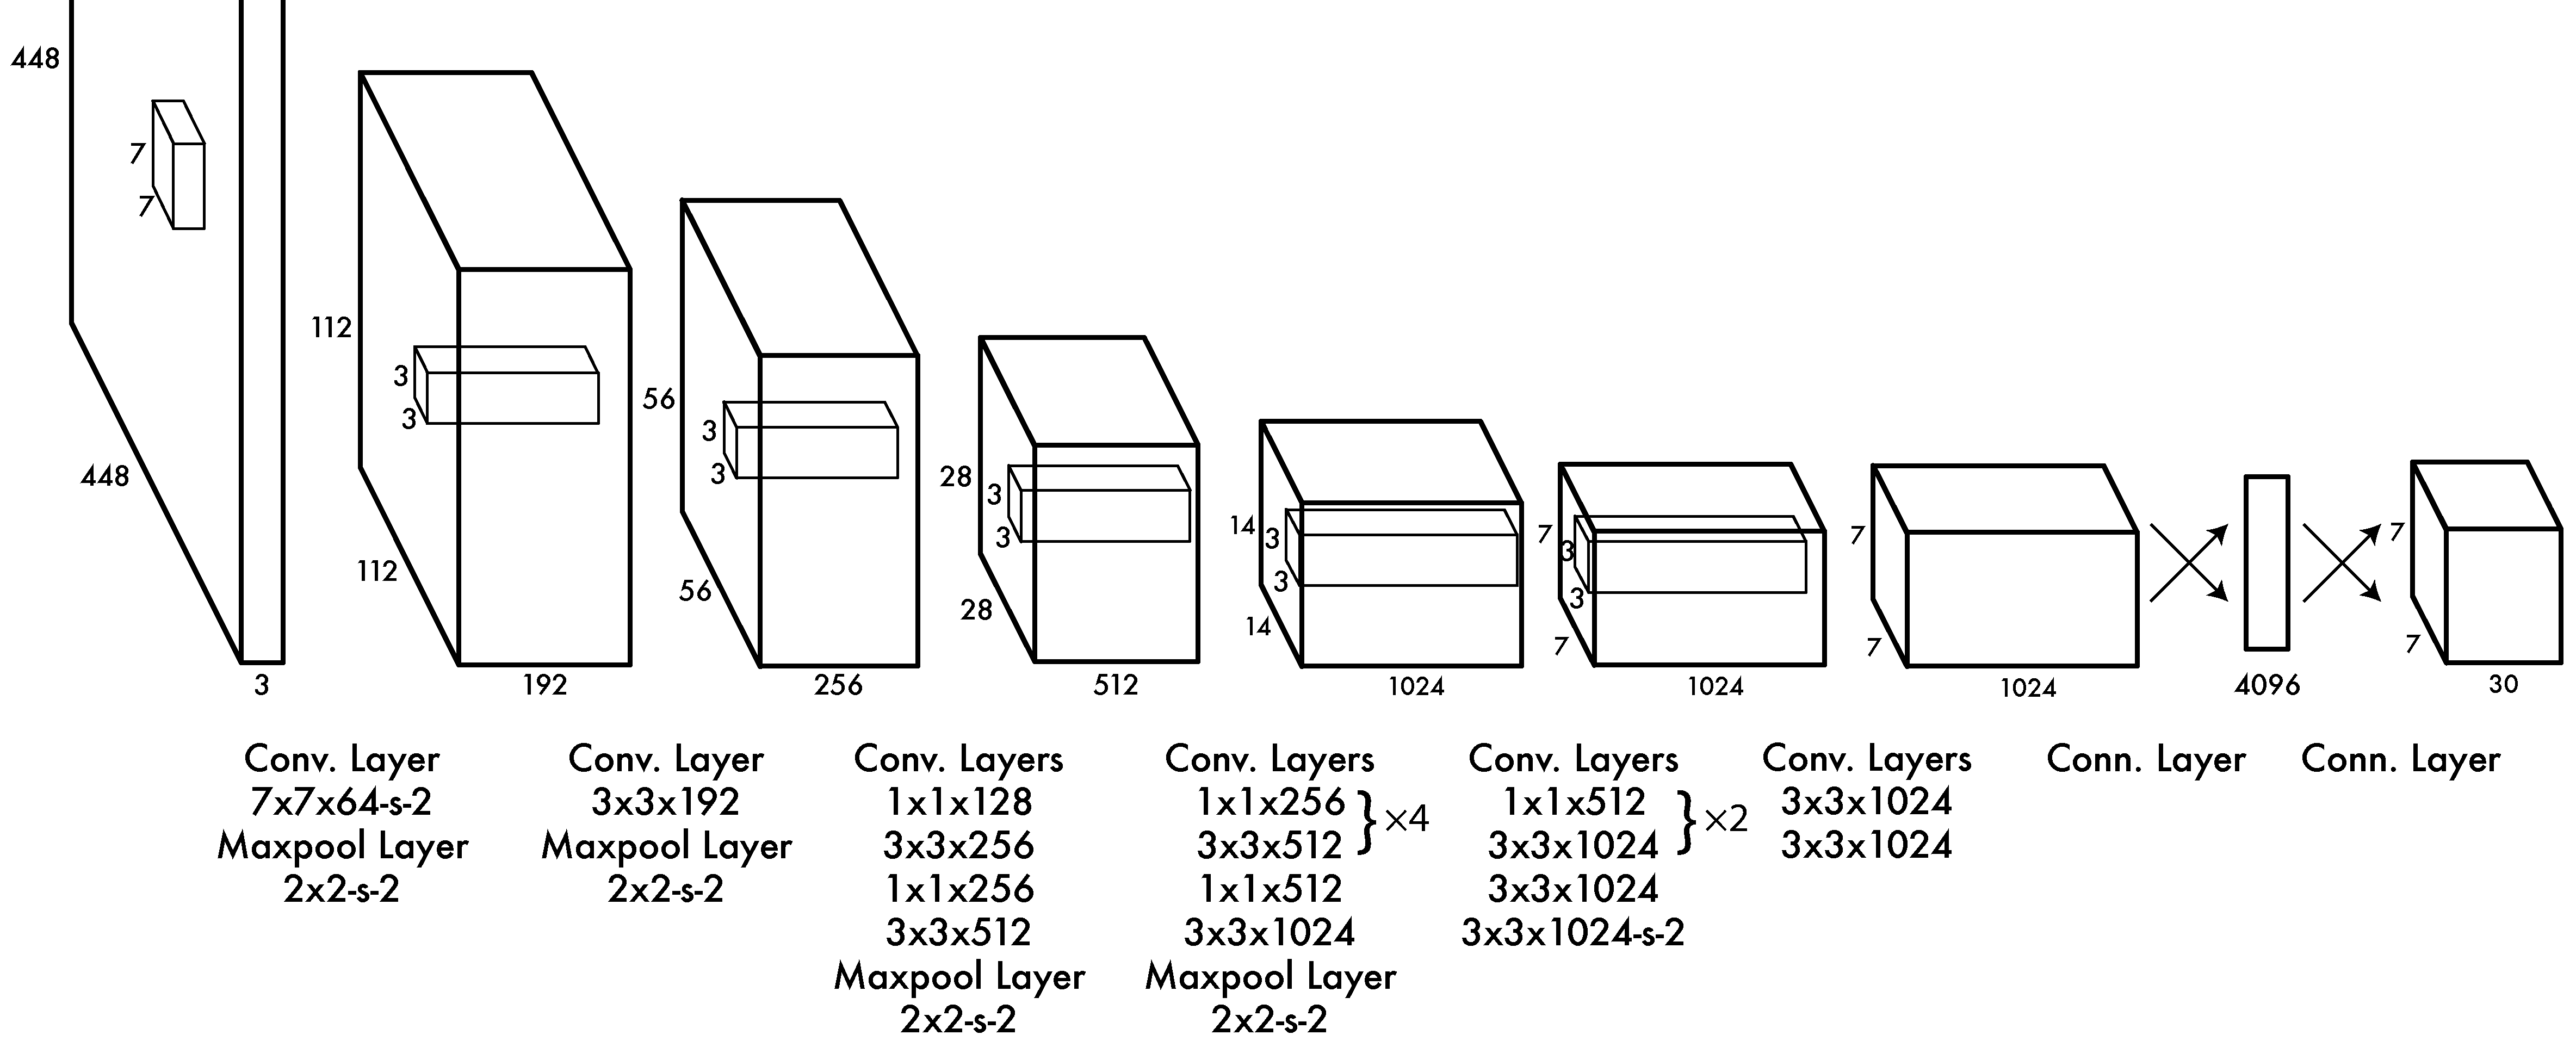
\includegraphics[width=0.8\textwidth]{Figures/yolo}
    \caption{Architektura původní verze YOLO \cite{yolo}}
    \label{fig:yolo}
\end{figure}

Každý bounding box je reprezentován souřadnicemi středu a velikosti (šířka a
výška). Dohromady s informací o jistotě detekce bounding boxu (confidence
score) vrátí model $5$ informací o každém bounding boxu. Pro každé pole mřížky
pak určí společnou informaci o třídě všech objektů v daném poli. Pokud objekt
není detekován, třída indikuje pozadí a souřadnice bounding boxu jsou
ignorovány. Velikost výstupního vektoru je tedy $7 \times 7 \times (2 * 5 +
    C)$, kde $C$ je počet definovaných tříd – v původní verzi pouze 20.

Tento algoritmus, navržený v roce 2015 J. Redmonem et al., byl revolučně
rychlý, zároveň v porovnání s jinými real-time detekčními algoritmy dosahoval i
slušné přesnosti. Nicméně byl velice citlivý na velikost objektu a přesnost
detekce, zejména u menších objektů, byla horší než u dvoufázových algoritmů.

Další verze algoritmu YOLO přinesly postupná vylepšení ve formě optimalizace
trénování a architektury. YOLOv2 \cite{yolo9000} zavedl mj. trénování na
několika měřítkách a byl natrénován s 9000 třídami (proto také nazýván
YOLO9000). YOLOv3 \cite{yolov3} přinesl mj. detekci na několika měřítkách.
Postupně byla také zvětšována mřížka a měnila se použitá architektura CNN sítě
sloužící pro extrakci příznaků pro jednotlivá pole mřížky \cite{yoloversions}.
Postupně také byly přidávány další funkce jako je segmentace, detekce pózy či
sledování objektů (ang. tracking).

V 2020 roce firma Ultralytics poprvé implementovala YOLO s využitím populární
knihovny PyTorch (YOLOv5), což umožnilo snadnější využití YOLO v praxi. Firma
Ultralytics také vytvořila framework pro použití různých verzí YOLO (YOLOv3 a
novější). Také pracuje na dalších vylepšeních a optimalizacích. Konkrétně
vytvořila YOLOv5 (2020), YOLOv8 (2023) a YOLOv11 (2024). Tyto verze nicméně
nejsou podloženy odbornými články, někteří je tak považují za neoficiální
verze.

\subsubsection*{SSD}
Dalším populárním algoritmem, který používá jednofázový přístup, je SSD (z ang.
single shot detector) \cite{szegedy:ssd}. Ten rozdělí vstupní obraz do několika
mřížek o různé velikosti. Postup je takový, že nejprve obraz projde konvoluční
sítí, konkrétně sítí VGG16, která extrahuje mapu příznaků. Tu se postupně
dalšími konvolučními vrstvami zmenšuje, výstup každého stádia zmenšení,
reprezentující mřížku dané velikosti, se spolu s původní mapou dále zpracovává
plně propojenou sítí.
\begin{figure}[]
    \centering
    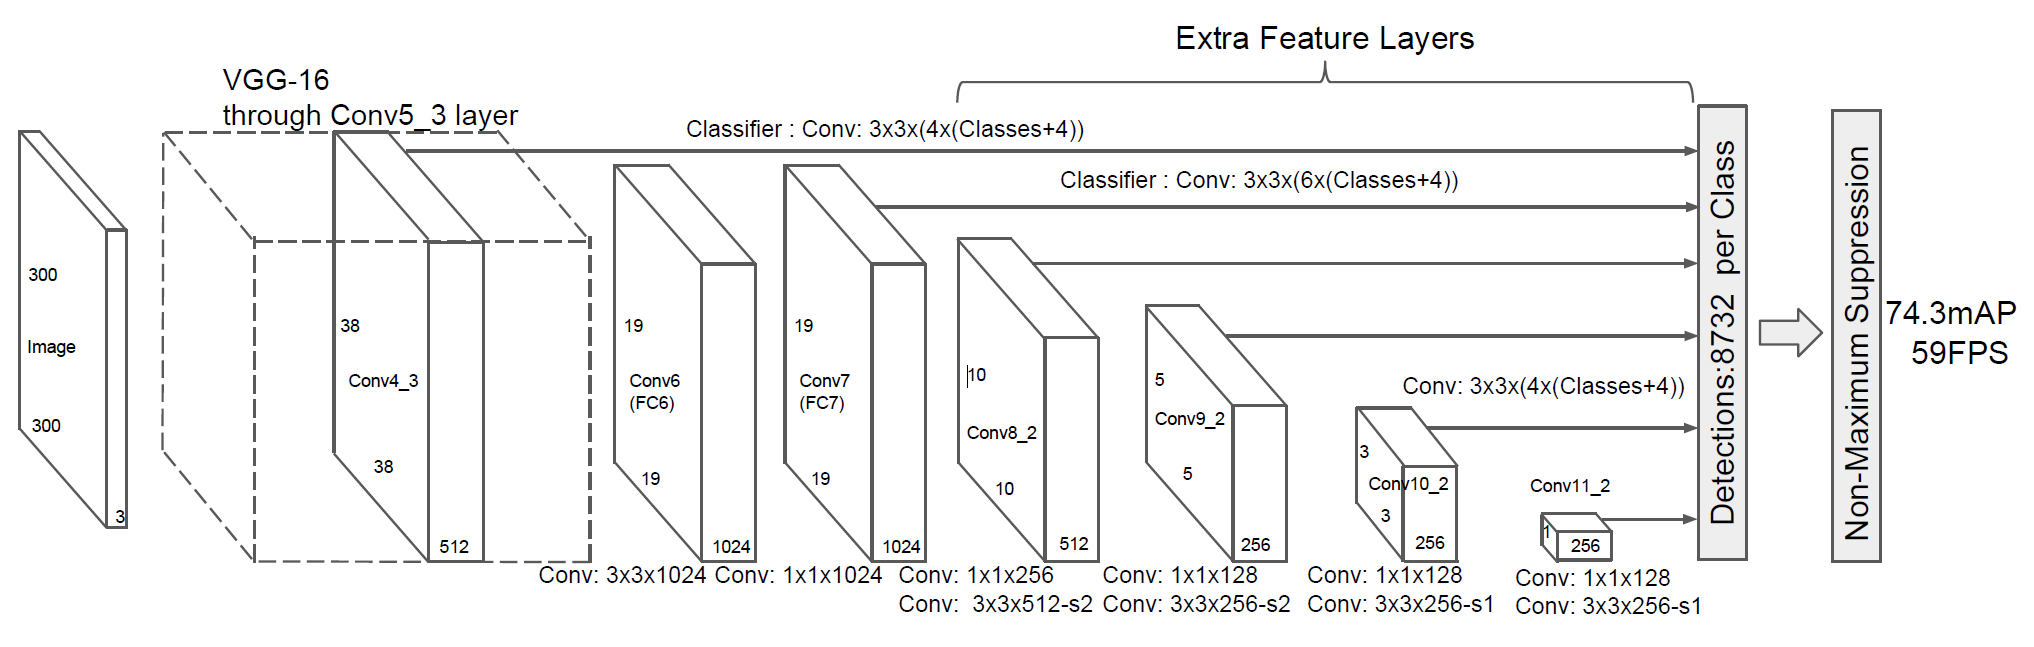
\includegraphics[width=0.8\textwidth]{Figures/ssd.png}
    \caption{Architektura SSD \cite{szegedy:ssd}}
    \label{fig:ssd}
\end{figure}

Výstupní bounding boxy nejsou, jako v případě YOLO, pouze výsledkem regrese,
ale pro každé pole dané mřížky je definováno několik výchozích oblastí (ang.
default box), ze kterých jsou vybrány ty, které obsahují objekt. K nim je
predikována třída objektu a posun i změna velikosti výchozí oblasti,
upřesňující výsledný bounding box.

V době svého vzniku byl SSD rychlejší a přesnější než YOLO, ale novější verze
YOLO jej už předběhly. Nicméně některé principy SSD, jako výchozí oblasti či
použití různých měřítek, byly převzaty do novějších verzí YOLO \cite{szegedy:ssd}.

\section{Charakteristiky vybraných implementací pro detekci pózy}

V této sekci bude popsáno několik populárních algoritmů (a jejich implementací)
pro detekci pózy, zejména se zaměřením na jejich rychlost, přesnost a specifika
architektury.

Velká část algoritmů byla zamítnuta a neproběhlo ani jejich testování.
Nejčastějším důvodem zamítnutí některého z algoritmů je, že schází jeho volně
dostupná, aktualizovaná implementace. Tvůrci algoritmů většinou investují čas a
zdroje pro vývoj algoritmu a natrénování modelu (často pro akademické účely),
pak ale neinvestují do jeho údržby. Zejména v prostředí Pythonu, kde se
neustále vyvíjejí nové knihovny a zpětná kompatibilita starších verzí není
zaručena, je pak obtížné použít takovéto řešení ve svém projektu, aniž by bylo
nutné investovat další čas do pochopení zdrojového kódu a jeho úpravy. Jak již
bylo zmíněno na počátku kapitoly, implementace algoritmu od nuly by vyžadovala
velké množství času a zdrojů (zejména výpočetních), hlavně by také byla
potřebná hlubší znalost problematiky. Někdy je možné řešení použít za cenu
kompromisu ve formě použití starších verzí knihoven či Pythonu, může to ale
představovat bezpečnostní rizika. Také některé algoritmy jsou sice volně
dostupné, ale jejich implementace jsou součástí komerčních produktů, např.
OpenPose, jež je mj. součástí produktu Viso Suite od viso.ai
\cite{visoai_openpose}.

\subsection{DeepPose}

DeepPose je historicky první algoritmus pro detekci pózy využívající hluboké
učení. Vyvinuli jej Alexander Toshev a Christian Szegedy ze společnosti Google
v roce 2014 \cite{deeppose}. Algoritmus předpokládá, že se ve vstupním obraze
nachází pouze jedna osoba. Síť se snaží v jednom kroku pomocí regrese jak
detekovat osobu, tak i její klíčové body. Jelikož je těžké takto dosáhnout
velmi přesných výsledků, algoritmus používá další fázi, která pomocí regrese
provádí posun bodů k přesnějším výsledkům. Tato fáze je aplikována opakovaně,
kaskádně se tak zvyšuje přesnost detekce.

Při svém vzniku byl DeepPose revoluční, nicméně v porovnání s dnešními řešeními
je poměrně pomalý a nepřesný. Nicméně položil základ pro využití hlubokého
učení v oblasti detekce pózy.

\subsection{OpenPose}

OpenPose \cite{openpose} je typicky příklad přístupu zdola nahoru. Jeho výhodou
je ale možnost vyhledání více osob v jednom snímku. Tento algoritmus, který
vyvinuli v roce 2019 Zhe Cao et al., nejprve pomocí CNN vytvoří heatmapu pro
každý typ klíčového bodu. Pro spojení bodů do jednotlivých osob využije pole
propojení klíčových bodů (ang. part affinity field – PAF). PAF je mapa
vytvořená pro každou končetinu (myšleno obecně spojení dvou klíčových bodů),
která v oblasti dané končetiny obsahuje hodnoty určující směr z jednoho bodu do
druhého. Pokud jsou pak spojené informace z heatmap a z PAF, je možné poměrně
jednoznačně zkompletovat jednotlivé klíčové body do celých postav. Stejně jako
heatmapy, jsou i PAF součástí trénovacích dat.

\subsection{OpenPifPaf}

Algoritmus OpenPifPaf \cite{openpifpaf}, vyvinutý v roce 2021 Svenem Kreissem
et al., je v podstatě vylepšenou verzí OpenPose. Jeho název je odvozen od dvou
stavebních kamenů: PIF (Part Intensity Field) – pole intenzity klíčových bodů,
a PAF (Part Affinity Field) – pole propojení klíčových bodů. PIF je rozšířením
heatmap, kdy kromě intenzity pravděpodobnosti klíčového bodu obsahuje i jeho
posun, zaručující přesnější lokalizaci bodu, a odhadovanou velikost dané části
těla. PAF v OpenPifPaf je také podobný tomu v OpenPose, navíc ale indikuje
kromě směru i velikost dané končetiny, což umožňuje lepší prostorové zachycení
pózy.

Dalším rozšířením oproti OpenPose je možnost sledování osob ve videu. Mapa
příznaků, která je výsledkem vstupní CNN, je udržována v mezipaměti, do další
části sítě pak vždy vstupují mapy pro aktuální a předchozí snímek. Výstupem pak
kromě klíčových bodů v každém snímku a jejich propojení tvořící kostru, jsou i
propojení mezi klíčovými body z jednotlivých snímků, viz
\ref{fig:pipaf-tracking}. Algoritmus si pak udržuje ID sledovaných osob, pokud
je k dříve nalezené osobě nalezena nová pozice, je jí přiřazeno stejné ID.
Pokud je nalezena nová osoba, je jí přiřazeno nové ID.

\begin{figure}[]
    \centering
    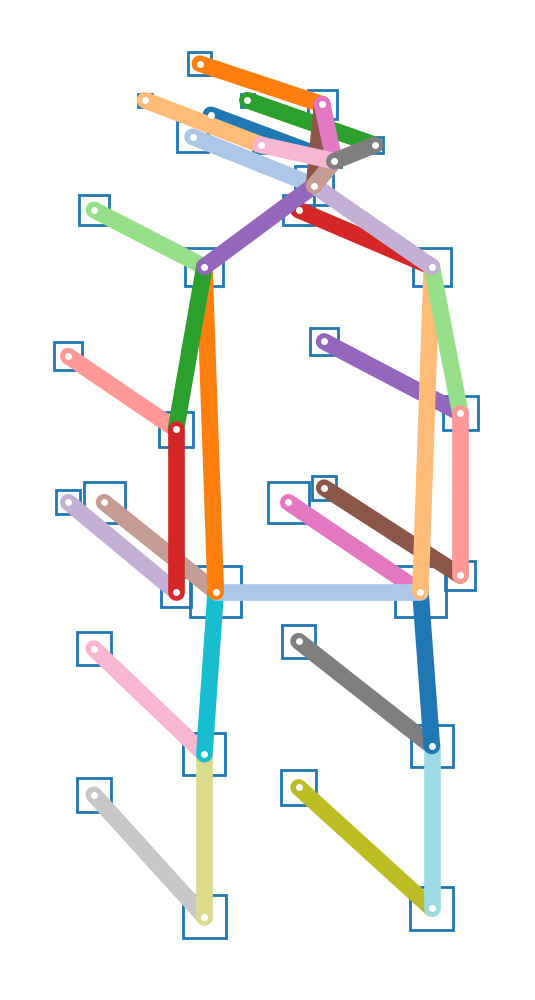
\includegraphics[height=0.2\textheight]{Figures/skeleton_forward2.png}
    \caption{Vizualizace  sledování osoby mezi dvěma snímky v OpenPifPaf \cite{openpifpaf}}
    \label{fig:pipaf-tracking}
\end{figure}

U OpenPifPaf je k dispozici výběr několika páteřních modelů, jako je ResNet50
či ShuffleNet v různých variantách a velikostech. Je tak možné zvolit model,
který je kompromisem mezi výkonem a přesností, v závislosti na konkrétních
požadavcích aplikace.

\subsection{MediaPipe – BlazePose}

MediaPipe je framework vyvinutý společností Google, umožňující jednoduchou
integraci různých technik strojového učení. Obsahuje různé algoritmy pro řešení
úloh jako detekce objektů, segmentace či detekce klíčových bodů (tváře či
pózy). MediaPipe je optimalizován pro mobilní zařízení a webové aplikace.
Detekce pózy v tomto frameworku je postavená na algoritmu BlazePose.

BlazePose implementuje přístup shora dolů, detekuje tedy nejprve RoI, ve
kterých detekuje osobu a její pózu. Nativně podporuje pouze jednu osobu ve
snímku. Ve videu ale v rámci optimalizace neprovádí detekci RoI pro každý
snímek, pouze pokud v aktuální RoI již není detekována osoba. Výhodou tohoto
algoritmu je, že detekuje 33 bodů v postavě, což je podstatně více, než většina
ostatních algoritmů, umožňuje tak přesnější analýzu některých situací, např.
podle natočení tváře, dlaní či stop.

Framework MediaPipe implementuje BlazePose spolu s detekcí více osob (v první
fázi používá detektor objektů). Výhodou tohoto frameworku je jeho kontinuální
vývoj a jednoduchost integrace. Nevýhodou ale je, že pro systémy Windows není
implementována podpora GPU. Jelikož výsledný produkt bude spouštěn primárně na
Windows zařízeních, je tato vlastnost rozhodující. Model je dostupný ve třech
velikostních variantách: $Lite$, $Full$ a $Heavy$.

\subsection{YOLO}

Od vydání YOLOv7 v roce 2022 integruje framework YOLO i detekci pózy. Oficiální
článek Chien-Yao Wanga et al. \cite{yolov7} sice neobsahoval tuto funkčnost,
ale oficiální implementace zahrnula i implementaci YOLO-Pose \cite{yolo-pose}.
Obecně detekce pózy v YOLO kombinuje přístup shora dolů a zdola nahoru.
Algoritmus sice vyhledává klíčové body spolu s bounding boxy osob, nicméně vše
v jednom kroku. Samotná detekce klíčových bodů využívá regresi, což
zjednodušuje proces trénování, jelikož není třeba tvořit heatmapy.

Architektura použitá v YOLO-Pose se ale liší od architektury používané v
pozdějších verzích. V YOLO-Pose jsou na konci řetězce umístěny hlavy pro různá
měřítka, jejich výstupem jsou bounding boxy a klíčové body, oba tvořené spolu.
V pozdějších verzích je architektura YOLO koncipována univerzálněji pro různé
úlohy. Obsahuje tak tři fáze\cite{yolov11}: páteř (ang. backbone), která
extrahuje mapu příznaků, krk (ang. neck), který přizpůsobuje mapu příznaků pro
různá měřítka, a hlavy (ang. head), které paralelně zpracovávají výstupy pro
různé úlohy, viz obrázek \ref{fig:yolov11} . Bounding box a klíčové body jsou
tedy sice generovány paralelně a teoreticky nezávisle, nicméně s ohledem na
proces trénování a postprocessing se v praxi navzájem výrazně ovlivňují.

\begin{figure}[]
    \centering
    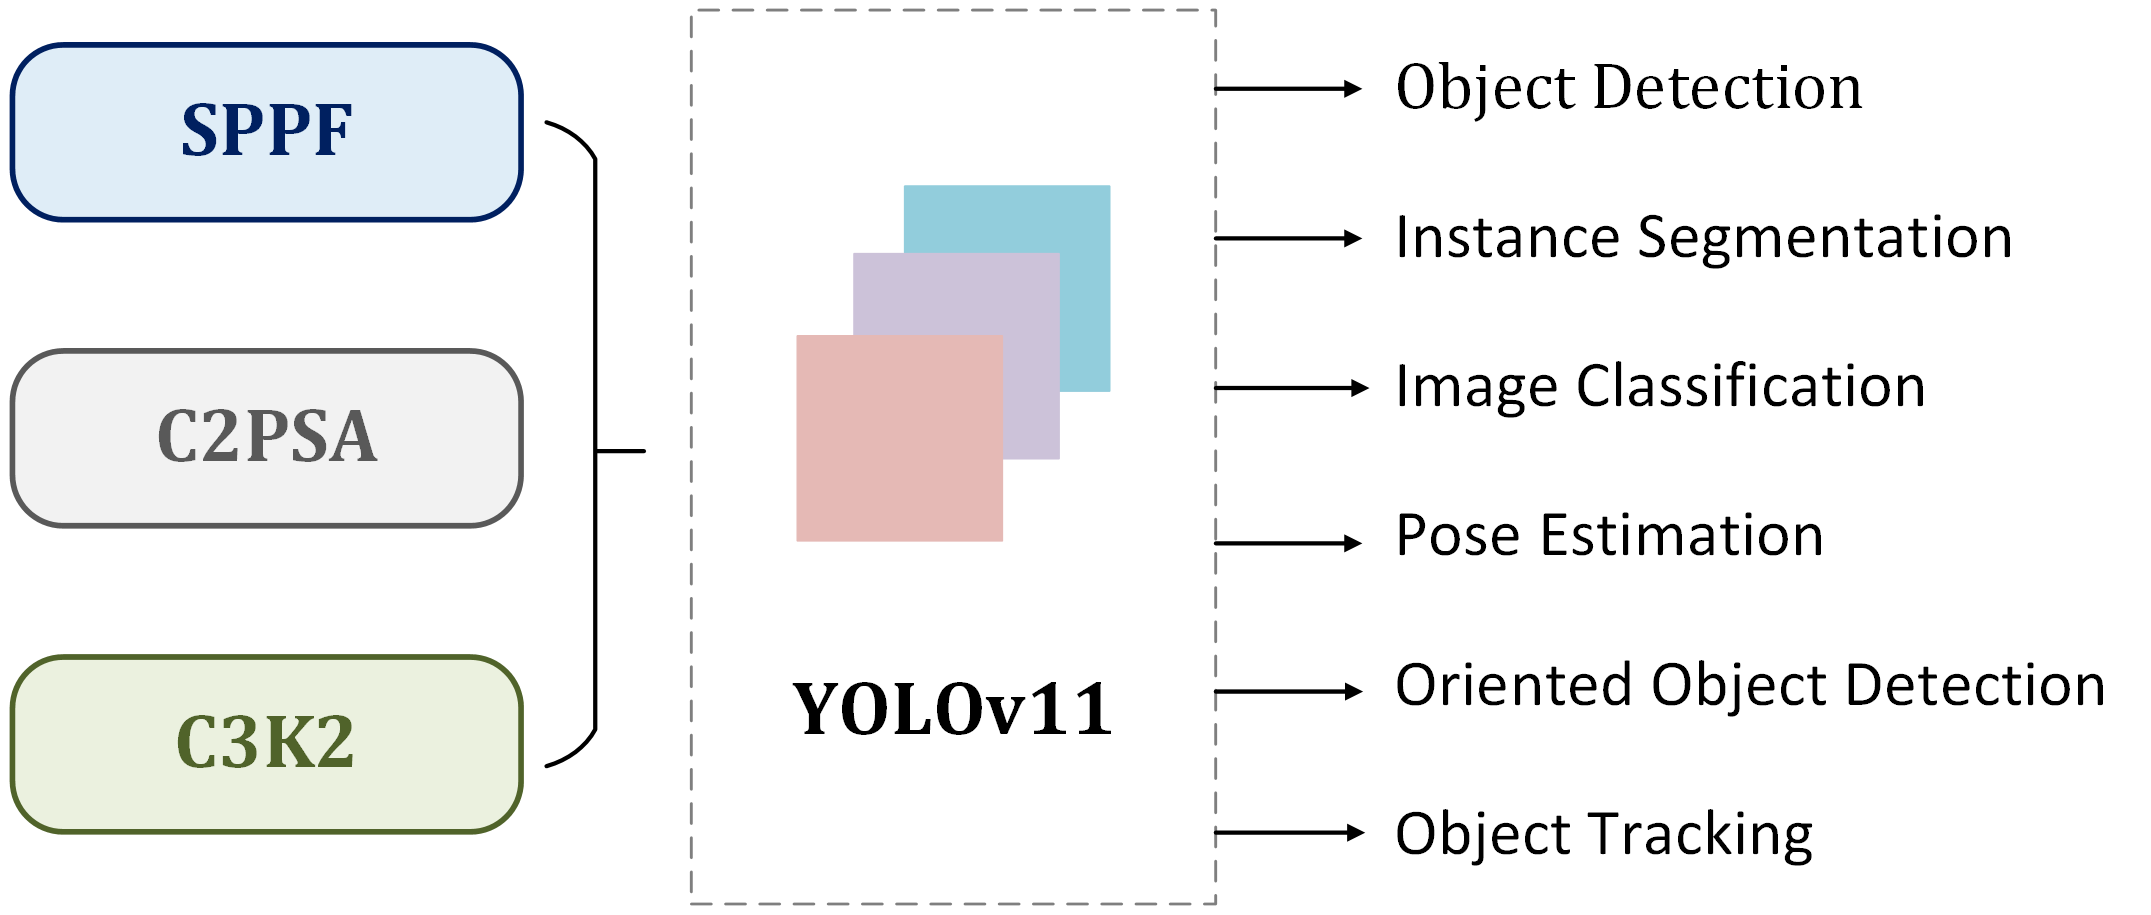
\includegraphics[height=0.2\textheight]{Figures/yolo_v11.png}
    \caption{Architektura YOLOv11 \cite{yolov11}}
    \label{fig:yolov11}
\end{figure}

Nejnovější verze YOLO také podporují kombinaci detekce klíčových bodů a
sledování osob. Model tedy kromě klíčových bodů vrací ID dané osoby, pomocí
kterého lze spojit danou postavu s předchozími snímky. Je tak možné efektivně
analyzovat pohyby jednotlivých osob.

Jednou z výhod framevorku YOLO, zejména verzí vyvíjených firmou Ultralytics, je
široká škála velikostí modelů. Každý model je dostupný v pěti variantách:
$Nano$, $Small$, $Medium$, $Large$, $Xlarge$.

\subsection{Torchvision}

Torchvision je knihovna, která je součástí frameworku PyTorch. Obsahuje různé
nástroje pro strojové vidění, jako je detekce objektů či segmentace. Její
součástí je i předtrénovaný model pro detekci pózy, který implementuje
algoritmus Keypoint R-CNN \cite{keypoint-rcnn}.

Algoritmus Keypoint R-CNN je založen na stejné myšlence jako Mask R-CNN
\cite{mask-r-cnn}, a tedy rozšíření Faster R-CNN o další hlavu, která v případě
Mask R-CNN provádí segmentaci, v případě Keypoint R-CNN detekuje klíčové body
\cite{keypoint-rcnn}. V algoritmu je také upravená pooling vrstva, která
zajišťuje, že se výstupy algoritmu shodují se vstupy s přesností pixelu.

Tato implementace bude testována zejména z důvodu její jednoduchosti použití a
integrace do frameworku PyTorch, který bude použitý i v další části řešení. Na
druhou stranu je oproti jiným frameworkům, jako je YOLO či MediaPipe, k
dispozici pouze jeden model, nikoliv více velikostních variant.

\section{Testování a porovnání vybraných algoritmů pro detekci pózy}

Pro testování byly vybrány čtyři algoritmy pro detekci pózy, zejména na základě
jednoduchosti jejich implementace, aktualizované podpory a požadovaných funkcí.
Testovány tedy budou algoritmy Torchvision, OpenPifPaf, MediaPipe BlazePose a
YOLO v nejnovější verzi 11. Testy byly provedeny na 25 videích ze stejného
datasetu jako byl použit později pro trénování algoritmu pro analýzu klíčových
bodů. Testování probíhalo na počítači s procesorem Intel Core i7, 32 GB RAM a
grafickou kartou NVIDIA GeForce RTX 3080 s 10 GB VRAM.

Algoritmy Torchvision a OpenPifPaf byly testovány s použitím GPU, MediaPipe
pouze s využitím CPU, jelikož v prostředí Windows nemá podporu GPU. Algoritmus
YOLO byl testován na GPU a CPU, pro porovnání jeho výkonu v různých podmínkách.
Algoritmus YOLO byl také vyzkoušen na GPU s využitím funkce sledování.

Výstupem testování pro daný algoritmus a jeho variantu je průměrná doba
zpracování jednoho snímku a videa s vykreslením klíčových bodů. Tato videa
dovolují ověřit schopnost detekce klíčových bodů v různých situacích a její
přesnost.

Následující část se věnuje výsledkům testování jednotlivých algoritmů. Pro
každý algoritmus budou porovnány jednotlivé varianty s ohledem na rychlost a
přesnost a budou vyhodnoceny jeho výhody či nevýhody oproti ostatním
algoritmům. Nakonec bude zvolen model, který bude použitý v další části vývoje.

\subsection{Výkonové požadavky}
\label{sec:performance_requirements}

Při výběru algoritmu je třeba s ohledem na práci v reálném čase brát v úvahu
zejména výkon detekčního algoritmu. Bezpečnostní kamery mají obvykle snímkovou
frekvenci od 15 do 30 snímků za sekundu (FPS), ideální by tedy bylo, aby
konečný program byl schopen pracovat s frekvencí alespoň 30 FPS. Zároveň se
předpokládá, že v prostředí, kde bude program nasazen, bude dostupná grafická
karta.

V této fázi již bylo zkoušeno trénování neuronové sítě pro klasifikaci pózy, a
bylo ověřeno, že i v případě hlubších a komplexnějších sítí je dosaženo doby
inference v řádu nižších jednotek milisekund. Hlavní vliv na výslednou rychlost
programu tedy bude mít hlavně detekční algoritmus, který musí zpracovávat
mnohem větší objem dat – stovky tisíc až miliony pixelů oproti např. 17
klíčovým bodům v případě klasifikačního algoritmu.

\subsection{OpenPifPaf}

Algoritmus OpenPifPaf byl zkoušen v několika variantách, postavených na síti
\textit{ResNet 50} a \textit{ShuffleNet V2} \cite{shufflenetv2}. V tabulce
\ref{tab:openpifpaf_performance} je vidět, že většina variant ani zdaleka
nedosahuje požadovaného výkonu.

Tento algoritmus je poměrně robustní z pohledu světelných podmínek a rozlišení
či rozmazaní obrazu, jinak ale dosahuje nejhorší přesnosti ze všech testovaných
algoritmů. Kromě nedetekování části těla, které nejsou vidět (jsou např.
schovány za jinou částí těla), totiž často nedetekuje člověka vůbec, nejčastěji
pak když člověk padá nebo leží, což jsou situace pro nás stěžejní. Hlavně tento
problém vystupuje ve variantě $resnet50$ a $shufflenetv2k16$, jsou tak pro
řešení nepoužitelné. Varianty $shufflenetv2k30$ a $tshufflenetv2k30$ by sice s
ohledem na kvalitu výsledků použitelné byly, nicméně je jejich výkon příliš
nízký.

\begin{table}[htbp]
    \centering
    \caption{Porovnání výkonu modelu OpenPifPaf}
    \label{tab:openpifpaf_performance}
    \begin{tabular}{|l|l|l|l|}
        \hline
        \textbf{Verze}   & \textbf{inference [ms]} & \textbf{Frekvence [FPS]} \\
        resnet50         & 49,2                    & 20.324                   \\ \hline
        shufflenetv2k16  & 31,3                    & 31.910                   \\ \hline
        shufflenetv2k30  & 58,6                    & 17.070                   \\ \hline
        tshufflenetv2k30 & 70,0                    & 14.281                   \\ \hline
    \end{tabular}
\end{table}

\subsection{MediaPipe BlazePose}

Algoritmus BlazePose z knihovny MediaPipe byl testován ve třech variantách:
$Lite$, $Full$ a $Heavy$. Ve všech variantách tento algoritmus dosahoval velmi
přesných výsledků, asi nejlepších ze všech testovaných algoritmů. Na rozdíl od
jiných algoritmů totiž, pokud detekoval osobu, vždy velmi přesně označil
všechny její klíčové body, v rámci možností i ty, které byly hůře viditelné
(např. schovány za jinou částí těla). Na obrázku \ref{fig:ym_comparison} je
vidět rozdíl v přesnosti detekce klíčových bodů mezi nejmenší variantou
BlazePose a druhou největší variantou YOLO, kdy BlazePose dosahuje mnohem větší
přesnosti, v tomto příkladě zejména co se týče detekce nohou.

\begin{figure}
    \centering
    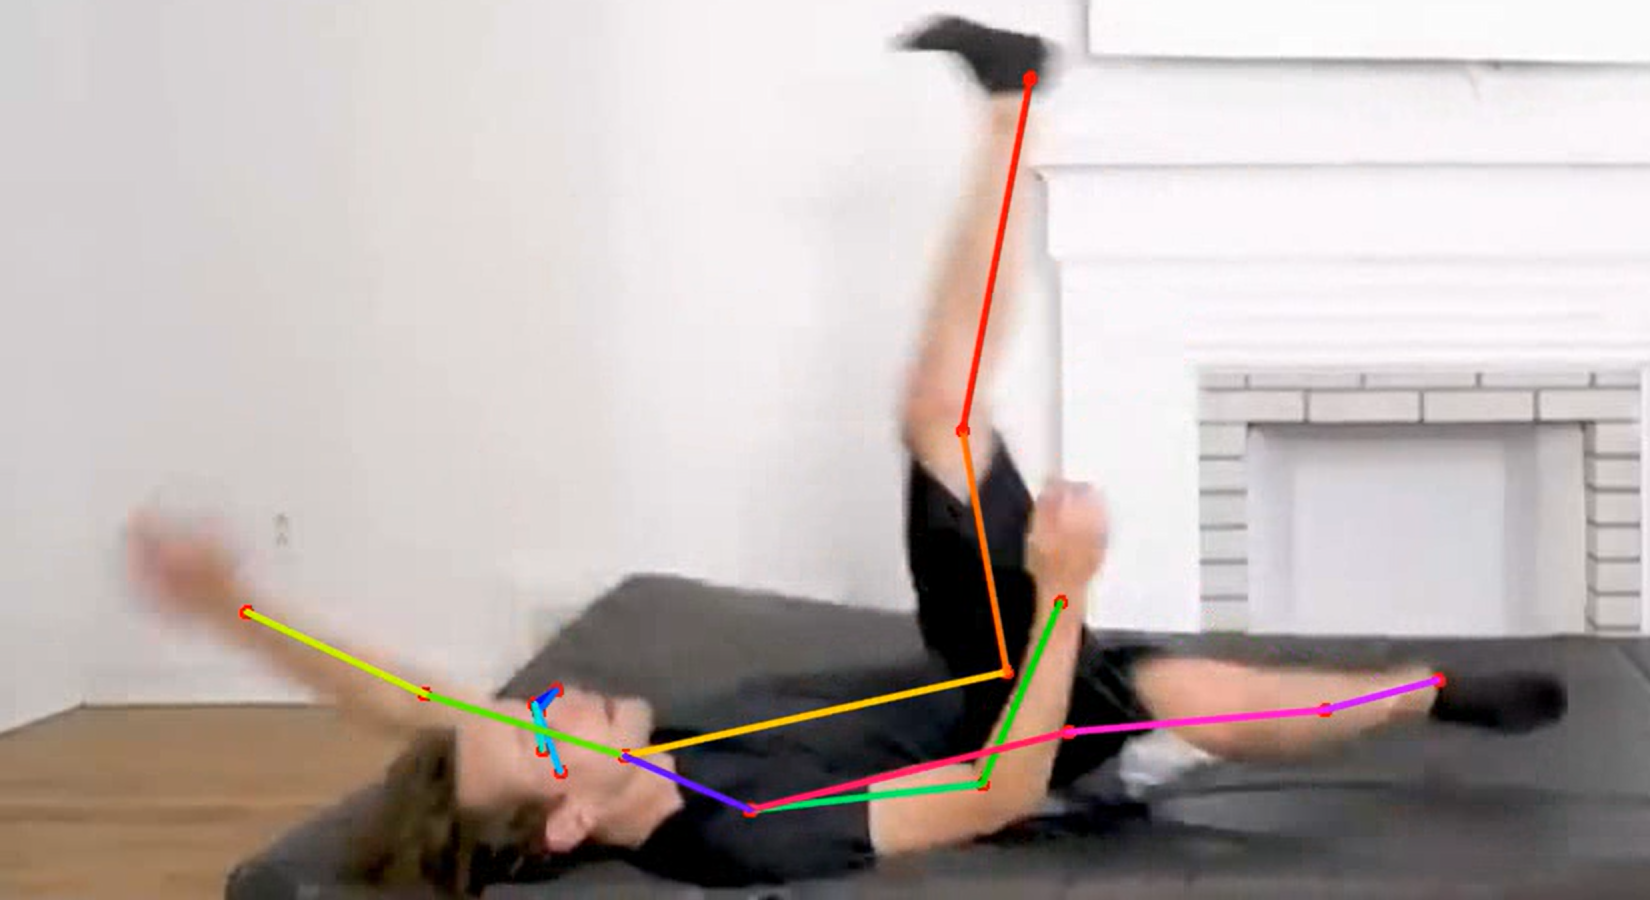
\includegraphics[width=0.4\textwidth]{Figures/pose_tests/mh1.png}
    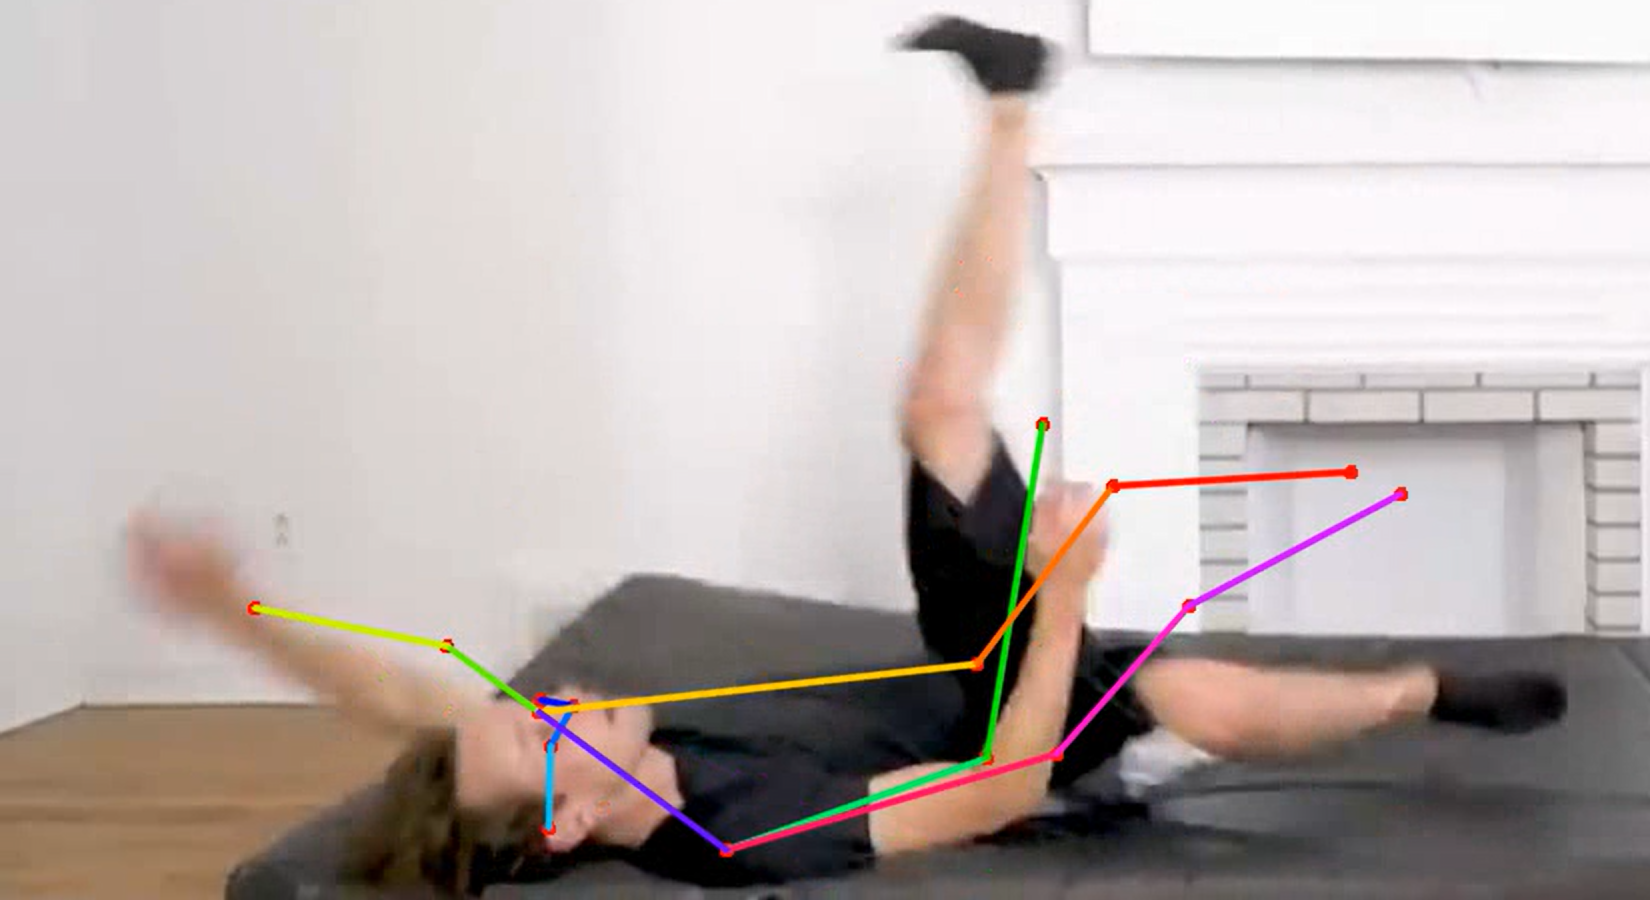
\includegraphics[width=0.4\textwidth]{Figures/pose_tests/yl1.png}
    \caption{Porovnání přesnosti \textit{MediaPipe Lite} (vlevo) a \textit{YOLO Large} (vpravo)}
    \label{fig:ym_comparison}
\end{figure}

S ohledem na to, že nemáme k dispozici grafickou akceleraci, je jeho výkon
velmi dobrý, viz tabulka \ref{tab:mediapipe_performance}. Verze $Lite$ a $Full$
by tak mohla být v našem řešení použitelná, což by nám také dávalo možnost
nasazovat výsledný program v mobilních zařízeních či jiných systémech bez
grafické karty.

\begin{table}[htbp]
    \centering
    \caption{Porovnání výkonu modelu MediaPipe BlazePose}
    \label{tab:mediapipe_performance}
    \begin{tabular}{|l|l|l|l|}
        \hline
        \textbf{Verze} & \textbf{inference [ms]} & \textbf{Frekvence [FPS]} \\
        \hline
        lite           & 25.5                    & 39.239                   \\ \hline
        full           & 30.9                    & 32.405                   \\ \hline
        heavy          & 68.2                    & 14.655                   \\ \hline
    \end{tabular}
\end{table}

Algoritmus si ale velice špatně radí s horšími světelnými podmínkami či menším
rozlišením obrazu. Ve většině případů sice detekuje klíčové body velmi přesně,
pokud je ale osoba hůř viditelná, nedetekuje ji vůbec. Tento problém se
projevuje ve všech variantách podobně. Jelikož bude výsledný program nasazován
spíše právě v podmínkách s horším osvětlením a ve větší vzdálenosti od osob,
pravděpodobně se pro aplikaci nebude hodit.

\subsection{Torchvision Keypoint R-CNN}

Torchvision Keypoint R-CNN nedosáhla ani dostatečného výkonu, viz tabulka
\ref{tab:torchvision_performance}, ani kvalitních výsledků. Podobně jako
\textit{OpenPifPaf} má totiž problém, když osoba padá anebo leží. V tomto
případě osobu často detekuje, ale naprosto ztrácí přesnost detekovaných
klíčových bodů, nejčastěji záměnou jednotlivých bodů, viz obrázek
\ref{fig:torchvision_bad}. Zároveň oproti BlazePose nemá takový problém s
horšími světelnými podmínkami a menším rozlišením obrazu.

\begin{figure}[]
    \centering
    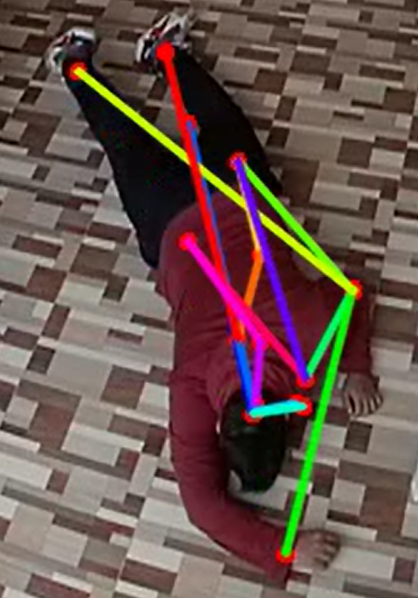
\includegraphics[width=0.2\textwidth]{Figures/pose_tests/torchvision_bad.png}
    \caption{Příklad špatné detekce bodů v modelu Torchvision Keypoint R-CNN}
    \label{fig:torchvision_bad}
\end{figure}

\begin{table}[htbp]
    \centering
    \caption{Výkon modelu Torchvision Keypoint R-CNN}
    \label{tab:torchvision_performance}
    \begin{tabular}{|l|l|}
        \hline
        \textbf{inference [ms]} & \textbf{Frekvence [FPS]} \\
        \hline
        50.3                    & 19.897                   \\ \hline
    \end{tabular}
\end{table}

\subsection{YOLO}

Algoritmus YOLO ve verzi 11 byl testován v pěti variantách: $Nano$, $Small$,
$Medium$, $Large$ a $Xlarge$. Všechny varianty byly testovány na GPU i CPU.

V tabulce \ref{tab:yolo_performance} je vidět, že na CPU dosahuje tento
algoritmus poměrně špatných výsledků. Jediný použitelný by mohl být v takové
situaci model $Nano$. YOLO je ale velice kvalitně optimalizováno pro grafické
karty, lze tak pozorovat, že na GPU je výkon výrazně vyšší. Pro potřeby řešení
by tak byly použitelné prakticky všechny varianty.

Jelikož pro analýzu více osob v jednom snímku je potřeba, zejména v případě
použití rekurentní neuronové sítě, jednotlivé osoby od sebe oddělit a
identifikovat i mezi snímky, bude velmi užitečná funkce sledování objektu.
Proto byl otestován algoritmus YOLO i s touto funkcí. Jak je vidět v tabulce
\ref{tab:yolo_performance}, je výkon sice horší než bez sledování, pořád ale
tři menší varianty dosahují frekvence větší než $30$ FPS.

\begin{table}[htbp]
    \centering
    \caption{Porovnání výkonu modelu YOLO}
    \label{tab:yolo_performance}
    \begin{tabular}{|c|l|l|l|}
        \hline
                                           & \textbf{Verze} & \textbf{inference [ms]} & \textbf{Frekvence [FPS]} \\
        \hline\hline
        \multirow{3}{*}{CPU}               & nano           & 32.5                    & 30.749                   \\ \cline{2-4}
                                           & small          & 53.9                    & 18.563                   \\ \cline{2-4}
                                           & medium         & 114.1                   & 8.763                    \\ \cline{2-4}
                                           & large          & 143.4                   & 6.973                    \\ \cline{2-4}
                                           & xlarge         & 833.2                   & 1.200                    \\ \hline\hline
        \multirow{3}{*}{GPU}               & nano           & 15.1                    & 66.323                   \\ \cline{2-4}
                                           & small          & 15.2                    & 65.972                   \\ \cline{2-4}
                                           & medium         & 17.4                    & 57.500                   \\ \cline{2-4}
                                           & large          & 24.4                    & 41.026                   \\ \cline{2-4}
                                           & xlarge         & 24.4                    & 41.005                   \\ \hline\hline
        \multirow{3}{*}{GPU se sledováním} & nano           & 27.4                    & 36.500                   \\ \cline{2-4}
                                           & small          & 27.7                    & 36.148                   \\ \cline{2-4}
                                           & medium         & 29.5                    & 33.882                   \\ \cline{2-4}
                                           & large          & 37.5                    & 26.664                   \\ \cline{2-4}
                                           & xlarge         & 40.5                    & 24.695                   \\ \hline
    \end{tabular}
\end{table}

Všechny varianty algoritmu YOLO dosahují poměrně kvalitních výsledků. I v
horších světelných podmínkách vždy detekují osobu, a víceméně přesně určí její
klíčové body. Obecně je ale vidět, že je model trochu méně robustní (než např.
MediaPipe) v situacích, kdy není dobře vidět některá končetina – je např.
schovaná za jinou částí těla, anebo ve specifických pózách – např. když je
osoba v dřepu nebo je v obraze natočená vzhůru nohama. V takovýchto případech
dosahuje menší přesnosti pro jednotlivé body – detekuje jiné natočení končetiny
nebo v extrémních případech špatně vyhodnotí natočení celé postavy. Špatně
viditelné části těla pak často vůbec nedetekuje.

Z pohledu přesnosti je zde výrazně vidět vliv velikosti modelu na přesnost
detekce. Varianta $Nano$ ve výše zmíněných situacích někdy detekuje body zcela
špatně, a je tak prakticky nepoužitelná. Varianta $Small$ je znatelně lepší,
pořád ale v horších podmínkách vyhodnocuje mnoho části těla špatně – např.
zamění nohy. Varianta $Medium$ je už výrazně lepší. Není sice ideální, ve valné
většině ale vyhodnotí všechny části těla správně i když ne z přesností několika
pixelů. Varianty $Large$ a $Xlarge$ jsou pak už velmi přesné, projevuje se to
ale znatelně menší rychlostí.

\begin{figure}
    \centering
    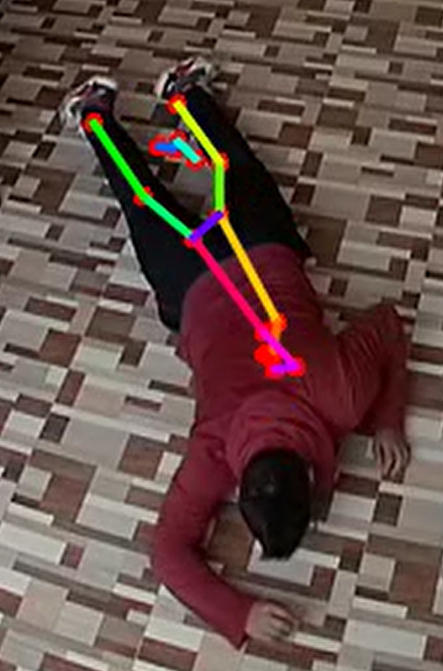
\includegraphics[width=0.18\textwidth]{Figures/pose_tests/y_n.png}
    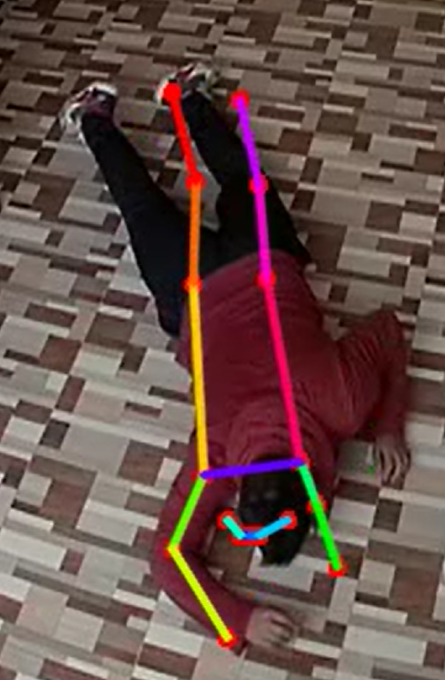
\includegraphics[width=0.18\textwidth]{Figures/pose_tests/y_s.png}
    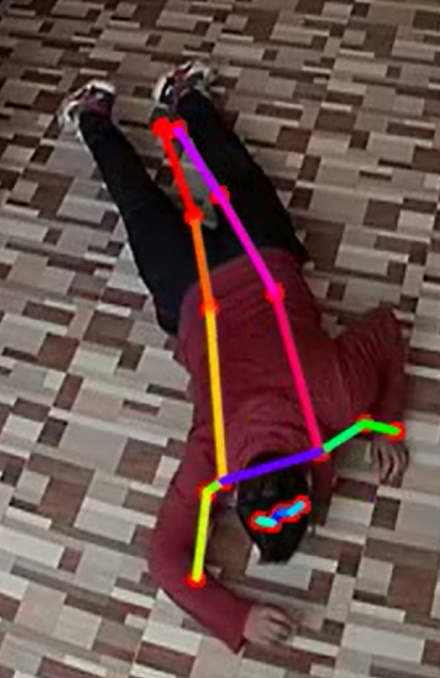
\includegraphics[width=0.18\textwidth]{Figures/pose_tests/y_m.png}
    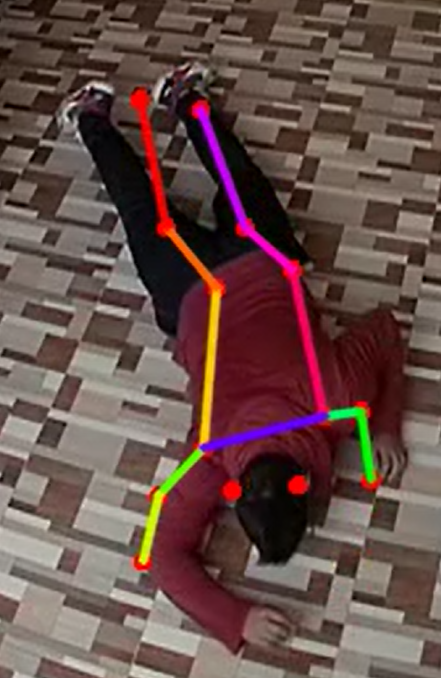
\includegraphics[width=0.18\textwidth]{Figures/pose_tests/y_l.png}
    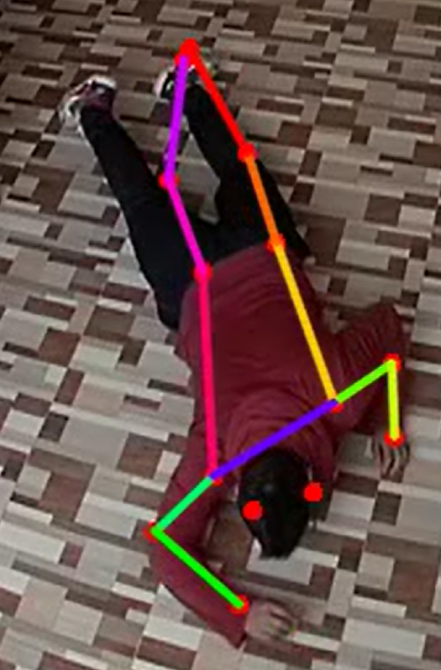
\includegraphics[width=0.18\textwidth]{Figures/pose_tests/y_x.png}
    \caption{Porovnání přesnosti variant modelu YOLO v situaci s netypickým natočením postavy. Zleva: $Nano$, $Small$, $Medium$, $Large$, $Xlarge$}
    \label{fig:y_comparison}
\end{figure}

Je zajímavé pozorovat, že i když je algoritmus BlazePose v mnoha situacích
mnohém přesnější, než i větší varianty YOLO, viz obrázek
\ref{fig:ym_comparison}, při horší viditelnosti, kdy i nejmenší varianty YOLO
detekují osobu, BlazePose zcela selhává. Ve snímku na obrázku
\ref{fig:y_comparison} například nedetekoval BlazePose osobu vůbec.

\subsection{Shrnutí a výběr modelu}

Z výše popsaného testování bylo zjištěno, že modely OpenPifPaf a Torchvision
jsou natrénované spíše pro detekci postavy, když je osoba v běžnějších pózách,
jako je ve stoje či chůze. Stejně i u menších variant YOLO přesnost prudce
klesá v méně typických pózách či natočeních v obraze. Jelikož ale je navrhované
řešení zaměřeno právě na detekování spíše netypické postavy, je pro nás
důležité detekovat pozici ve všech situacích.

Naopak algoritmus BlazePose je velmi přesný, strádá ale při horší viditelnosti
osoby. Nehodí se tak pro naše využití s kamerami s horším rozlišením a vysokou
vzdáleností od osob. Ostatní algoritmy jsou v tomto ohledu mnohem robustnější,
nejlépe si s horšími podmínkami poradí algoritmus YOLO.

Optimální cesta se tedy zdá být algoritmus YOLO ve verzi $Medium$, který
dosahuje dostatečné rychlosti i při sledování osob, zároveň dostatečně přesně
detekuje pózy ve všech pozicích i podmínkách. Pokud by nebyla pro analýzu pózy
použitá rekurentní neuronová síť, nemuselo by být nutné používat funkci
sledování a bylo by tak možné použít i větší variantu YOLO, což by mohlo
zlepšit přesnost detekce.

\endinput